\chapter{Verwandte Arbeiten} \label{sec:VerwandteArbeiten}
In diesem Abschnitt werden verwandte Arbeiten vorgestellt.
Im gegensatz zu dem literatur abschnitt werden wir hier nur Arbeiten vorstellen, die eine ähnliche Problemstellung haben, wie die in dieser Arbeit vorgestellte.
1. also vergleich von verschiedenen 2.5D visualierungen zur Software qualitäts visualisierung
2. verbesserung des Treemap Problems durch margins



\section{Vergleich von 2.5D Visualisierungen}



Das Paper vergleicht fünf dynamische Visualisierungstools hinsichtlich ihrer Unterstützung für Softwareverständnis und Reverse Engineering. Ziel ist es zu untersuchen, warum solche Tools kaum außerhalb der Forschung eingesetzt werden, obwohl sie grundsätzlich große Potenziale für das Verständnis und die Analyse von Softwaresystemen bieten. \textit{A comparative evaluation of dynamic visualisation tools} \cite{pacione2003comparative} 
altes paper 2003 
ziel ist für entwickler, anders als dieses paper
Ergebnisse Kein einziges tool reicht komplett aus
Tools sollten stärker Design Patterns sowie Hotspots - ziel dieser arbeit


5. An overview of 3D software visualization \cite{overview3D}
Der Artikel bietet einen umfassenden Überblick über den Stand der Forschung im Bereich 3D-Softwarevisualisierung. Ziel ist es, Methoden, Visualisierungsansätze, Interaktion, Tools und Evaluationsmethoden vorzustellen
Sie stellen viele verschiedene Ansätze vor und kategorisieren diese: Graphen: 3D-Knoten/Kantennetze z.B. zur Darstellung von Klassenbeziehungen, oft mit ausgefeilten Layout-Algorithmen (z.B. Kräfte-basiert, hyperbolische Layouts).
Bäume: 3D-Kegel-Bäume („Cone Trees“), Informationen als verschachtelte Container (z.B. „Information Cubes“).
Geometrische Primitive: Polyeder, Lego-Steine, Geons (primitive 3D-Formen), Metaballs u.a. als Darstellung von Softwarestrukturen.
Reale Welt-Metaphern:
Beispiele: „CodeCity“ (Software als 3D-Stadt), orbitale/solare Modelle, Landschaften, Molekül- oder Netzstrukturen, Game-Engines zur Darstellung von Code.
Interesant von 22 tools nur 4 für managers oder stakeholders bestimmt und davon nur 1 die auch die software visualiert, die anderen 3 geht es um requirements visualisierung. -> wenig ausgeprägt 
Sie stellen fest: Es gibt noch relativ wenige empirische Nutzungsstudien zu 3D-Visualisierung.




3. Visualization of the static aspects of software: A survey \cite{staticSurvey}
Ähnlich wie paper zuvor überblick geben
Quellcode-Ebene: Zeilenweise Ansichten wie SeeSoft oder sv3D
Klassen/Mittel-Ebene: Visualisierung der Inneren Struktur und Beziehungen einer oder mehrerer Klassen (z.B. Class Blueprint)
Architektur-Ebene: Überblick über die globale Organisation, Beziehungen (z.B. Erbe, Aufrufe), und Qualitätsmetriken der gesamten Software
für diese ebene stellen sie diese visualisierunge vor:
Tree/Node-Link Diagramme: Für kleine Hierarchien geeignet, werden bei großen Systemen aber schnell unübersichtlich.
Treemap, Circular Treemap, Sunburst, Voronoi Treemap: Platzsparende, hierarchische Darstellungen (Rechtecke, Kreise, Voronoi-Flächen), sowohl in 2D als auch 3D.
In dieser arbeit hier wird eher auf architektur ebene geschaut. da für kunden details nicht so wichtig sind, es geht um den überblick
Herausforderungen und offene Probleme:
Usability, Kognitive Überlastung, Disorientierung in 3D, Informationsüberladung
Geringe Verbreitung leistungsfähiger Tools in der Praxis (viele Forschungsprototypen)


6. Visualization and evolution of software architectures \cite{visualizationEvolution}
auch ähnlich wie paper zuvor überblick geben
Unterscheiden auch in hierarchische und beziehungsbasierte Visualisierungen. unss interessiert hier vorallem die hierarchischen Visualisierungen, da diese auch in dieser Arbeit verwendet werden:
Viele Softwarearchitekturen sind hierarchisch organisiert (Packages → Klassen → Methoden).
Klassische Node-Link-Diagramme (Knoten-Kanten-Diagramme) werden schnell unübersichtlich bei großen Systemen.
Treemaps: Platzfüllende, verschachtelte Rechtecke stellen Hierarchien kompakt dar, jedoch meist nur für Blätter geeignet; oft nur eine Metrik kann visualisiert werden.
Icicle Plots und Sunburst-Diagramme: Zeigen Hierarchien linear (Icicle) oder radial (Sunburst) an, erlauben Darstellung von zwei Metriken.
Hyperbolische Bäume: Nutzen eine verzerrte Geometrie, um mehr Informationen zentral sichtbar zu machen.




\cite{bassil2001software}
systematisch herauszufinden, welche funktionalen, praktischen und kognitiven Aspekte Nutzer an diesen Tools besonders schätzen, welche Probleme auftreten und welche Verbesserungswünsche bestehen.
Ergebnis: wichtig: Hierarchische Repräsentationen, Benutzerfreundlichkeit/Usability, Effizienz bei großen Systemen, Qualität der Benutzeroberfläche, .... noch mehr
wenige tools können: Berechnung von Metriken
aber auch für experten eher ausgerichtet


Erste Suche: allintitle: "3D Software Quality Visualization"
gibt nur ein relevantes Ergebnis:
The Visualization of Software Quality Metrics-A Systematic Literature Review
- bachelor thesis und nicht so viel zitiert
- aber gute grundlage trotzdem 
- nochmal lesen


durch literatur recherche gefunden: VON https://hpi.de/doellner/publications.html :
Scheibel et al. stellen in ihrem Paper \textit{Survey of treemap layout algorithms}\cite{scheibel2020survey} eine Übersicht über die verschiedenen Treemap Layout Algorithmen vor. Sie unterscheiden zwischen den verschiedenen Ansätzen. 

Sie kategorieren die verschiedenen Ansätze in 4 Kategorien: Art der Aufteilung, zusätzliche Attribute, Layout Form und Referenzraum Dimension. 
Uns interresiert hier besonders das zusätzliche Attribut der "Werte" und die Dimension 2D (wie in Abschnitt \ref{sec:Problemstellung} beschrieben).
Arten der Aufteilung sind: Packing und splitting. Packing ist dabei die Idee, die Knoten so zu packen, dass sie möglichst wenig Platz verbrauchen und splitting ist die Idee Knoten in kleinere Knoten zu unterteilen. Alle in den Grundlagen (Abschnit \ref{sec:Treemap}) vorgestellten Algorithmen sind also splitting Algorithmen.
Sie stellen vier Layout Formen vor: Kreisförmig, rechteckig, konvex und nicht konvex. Alle in den Grundlagen vorgestellten Algorithmen sind rechteckige Layouts.
Von den untersuchten 81 Algorithmen sind 54 rechteckige Layouts und 58 splitting Algorithmen. Der in dieser ARbeit speziell untersuchte Treemap Algorithmus passt also genau in die Kategorie der meist verwendeten Ansätze.


\section{Treemap Problem verwandte Arbeiten}
Wir suchen hierfür speziell nach layouts die abstände haben. die meisten treemap layouts haben keine abstände, wodurch bei der extrusion ins drei dimensionale und ohne farbgebung die Struktur der Hierarchie nicht mehr erkennbar ist. Deswegen wird speziell nach treemap layouts gesucht, die abstände haben und die Struktur der Hierarchie darstellen.


Aktuell gibt es nur eine arbeit die dieses Problem explizit anspricht und zwar \cite{lu2008cascaded}.


\cite{lu2008cascaded}:
Hao Lü and James Fogarty stellten in ihrem Paper \textit{Cascaded Treemaps:
Examining the Visibility and Stability of Structure in Treemaps}\cite{lu2008cascaded} fest: \enquote{an important limitation of treemaps is
the difficulty of discerning the structure of a hierarchy}\cite[1]{lu2008cascaded} Das stellt im Grunde das Problem von Treemaps dar, welches auch algorithmisch nicht einfach gelöst werden kann (siehe Abschnitt \ref{sec:TreemapProblem}). Die Idee ist anders als bei Nested Ansätzen die Kindknoten nicht einfach in den Elternknoten zu zeichnen, sondern sie leicht versetzt \textit{über} dem Elternknoten zu zeichnen (siehe Abbildung \ref{fig:cascaded}). Dadurch soll weniger Platz verloren gehen und es entsteht ein leichter 3D-Effekt.

\begin{figure}
    \centering
    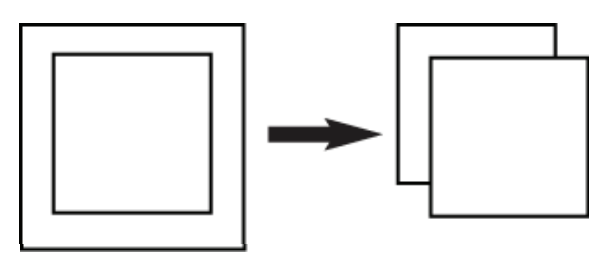
\includegraphics[width=0.8\textwidth]{images/cascaded.png}
    \caption{Links beispielhaf der Nested treemaps Ansatz, bei dem der Kindknoten einfach in dem Elternknoten gezeichnet wird. Rechts der Cascaded Treemap Ansatz, bei dem der Kindknoten als rechteck leicht versetzt nach rechts unten \textit{über} dem Elternknoten gezeichnet wird. Abbildung aus \cite[3]{lu2008cascaded}.}
    \label{fig:cascaded}
\end{figure}

Sie stellen in ihrem Paper auch fest, dass manche Knoten verschwinden können, da der Platz der für Beschriftung und abstände benötigt wird, beim Layoutschritt nicht berücksichtigt werden kann. Sie stellen einen Zwei Schrittigen ansatz vor, der im ersten schritt mit den squarify algorithmus \cite{bruls2000squarified} das layout erstellt. 
Im zweiten Schritt wird dann die Größe, aber nicht die Platzierung der Knoten angepasst. 
indem der Abstand und platz für Beschriftung berücksichtigt wird. Das Problem von verschwindenden Knoten wird dadurch nicht komplett gelöst, aber Knoten verschwinden nur noch, wenn der Platz für die Beschriftung und den Abstand größer ist als der zur Verfügung stehende Platz. Die Autoren geben leider keinen Pseudo-Code für die exakte implementierung an, weshalb es schwer ist die genaue berechnung nachzuvollziehen und Unterschiede und Vor- und Nachteile zu den Implementierungen in diser Arbeit aufzuzeigen.
Sie beschreiben ihren Schritt wie folgt: 
\begin{quote}
    The function then computes how much vertical space is needed for offsets [...]. The remaining space is for the content of the treemap, and so the layout function gives each side of the split the space computed as necessary for [...] offsets as well as a portion of the remaining content space based on the relative weights of nodes on each side of the split. The layout procedure is then ready to recurse on both sides of the split, as it knows how much space will be used by [...] offsets and has ensured that the remaining space is appropriately divided by node weight. \cite[6]{lu2008cascaded}
\end{quote} (FÜR MICH: das ist quasi simple-increase mit scaling)
Sie berechnen also die Fläche, für jeden Knoten neu. An jeder Teilungs-Kante, die kante an der ein Knoten geteilt wurde (entweder horizontal oder vertikal) - im grunde werden sich immer die reihen angeschaut. Wird dann der Platz berechnet, der für die Abstände benötigt wird. Anschließend wird der Platz für die Knoten berechnet, indem der Platz für die Abstände von der Gesamtfläche abgezogen wird. Dadurch wird sichergestellt, dass jeder Knoten genug Platz für die Abstände hat. Dennoch kann es passieren, dass Knoten verschwinden, wenn der Platz für die Abstände größer ist als der Platz, der für die Knoten zur Verfügung steht.
Obwohl der Code nicht verfügbar ist, wird doch allein bei der Beschreibung ein Nachteil deutlich: Es wird an jeder Reihen-Kante nur der Platz mit in die Berechnung einbezogen, der senkrecht zu der Kante steht. In Abbildung \ref{fig:cascadedBadExample} für deutlich, dass der Algorithmus für den Bereich über von der Kante benauso viel Platz für die Abstände berechnet, wie für den Bereicht unter der Kante, weil eben nur der Platz senkrecht zur Kante betrachtet wird. Und das obwohl offentlich die Roten Rechtecke zusammen viel Mehr platz für die Abstände benötigen würden, als das Gelbe Rechteck alleine. 
Das Grundlegende Problem, welches wir zuvor beschrieben haben (siehe Abschnitt \ref{sec:TreemapProblem}), ist also nicht gelöst. 

\begin{figure}
    \centering
    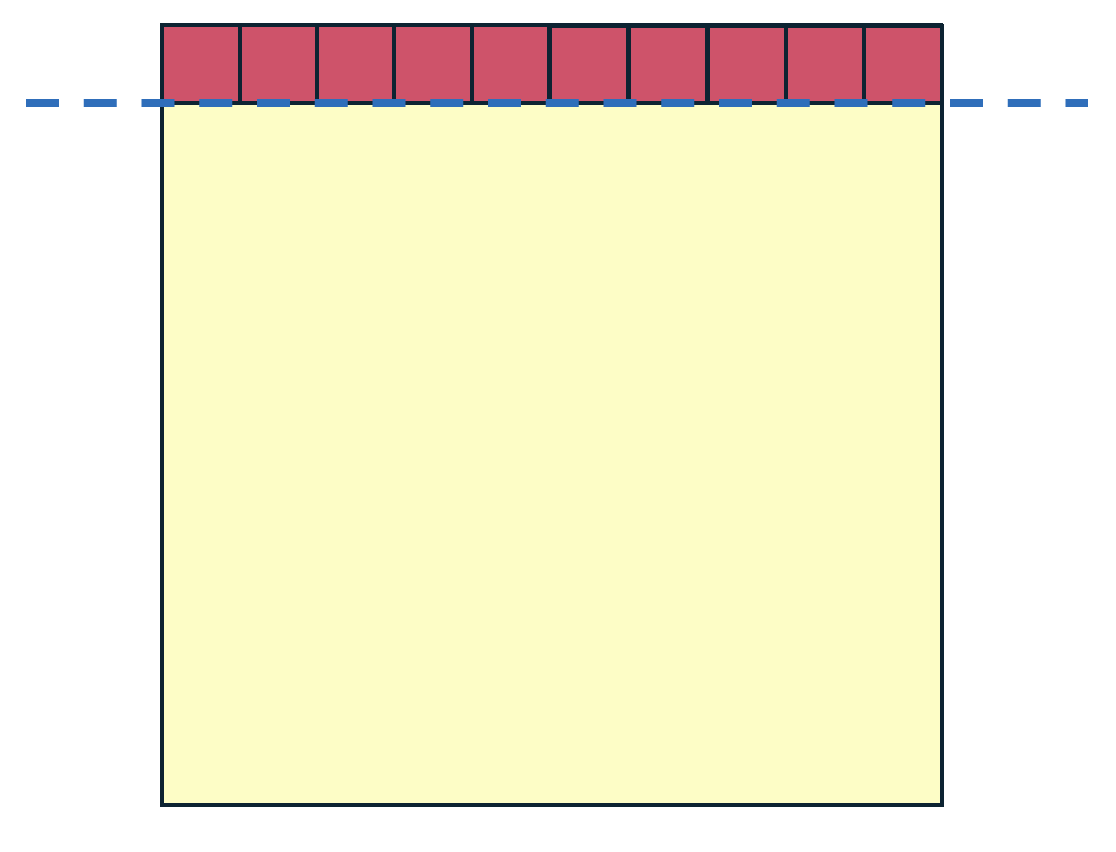
\includegraphics[width=0.8\textwidth]{images/cascadedBadExample.png}
    \caption{Beispiel für eine für den Cascaded Treemap Algorithmus schlechte Rechteck-Konstelation}
    \label{fig:cascadedBadExample}
\end{figure}

Interessant ist, dass die Autoren keine verbesserung in der Gewicht zu Größe relation feststellen konnten. (Ich vermute, dass das daran liegt, dass die Berechnung der neuen Größen für die Knoten nicht optimal ist) 
Eine verbesserung konnten sie nur bei relativ kleinen Knoten feststellen, was auch klar ist, da bei den ansätzen zuvor die Abstände (da diese ja absolut sind und bei jedem knoten gleich) die Größe von kleinen Knoten viel stärker beeinflussen, als die Größe von großen. Sie vermuten auch, dass das an Ihrem Ansatz speziell liegen könnte und fordern noch weitere research in diesem Bereich.
Sie vermuten außerdem, dass speziell bei Tiefen Hierarchien, die Abweichung von Größe zu Gewicht größer wird.  

Eine ähnliche implementierungen untersuchen wir in Abschnitt HIER EINFÜGEN und zeigen genau auf, warum dieser Ansatz große Schwächen hat. bzw 
Am ehesten ist dieser Ansatz wahrscheinlich mit dem Simple-Increase Ansatz mit Scaling und festen Knoten zu vergleichen, nur mit dem Umterschied, dass die kompletten abstände betrachtet werden und diese betrachtung nur einmalig nach dem ersten squarify Layout Schritt durchgeführt wird (was auch in dem casced paper angemerkt wurde, dass das einmalige berechnen der Abstände eine mögliche Optimierung ihres Ansatzes wäre \cite[6]{lu2008cascaded}).





Die Autoren des ursprungs squarify Algorithmus \cite{bruls2000squarified} stellen in einem anderen Paper \cite{cushionTreemaps} eine Idee vor, um Struktur ohne Änderung des Layouts darzustellen undzwar mit Schatten (siehe Abbildung \ref{fig:cushion}). Dabei bekommt jeder Knoten, egal ob Eltern- oder Kindknoten, einen Innenrenschatten, wodurch die Struktur der Knoten sichbar wird.

\begin{figure}
    \centering
    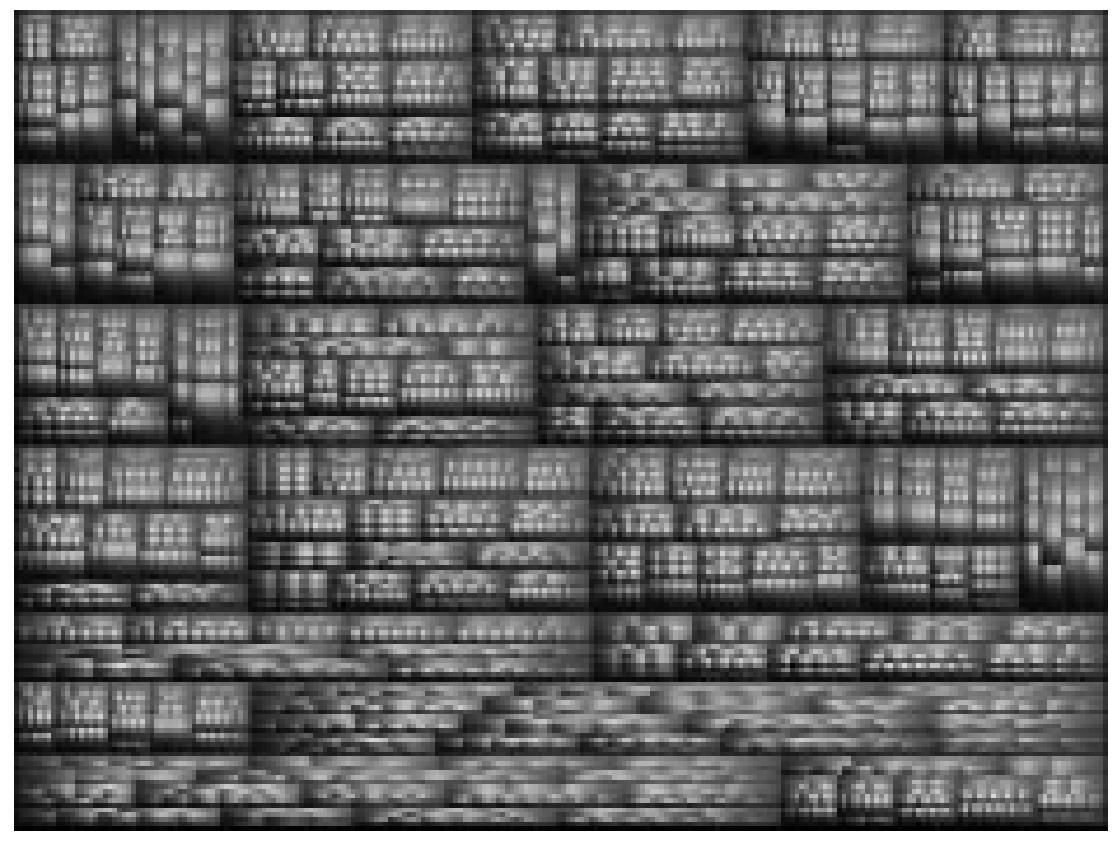
\includegraphics[width=0.8\textwidth]{images/cushionTreemap.png}
    \caption{Beispiel für eine Cushion Treemap \cite[4]{cushionTreemaps}}
    \label{fig:cushion}
\end{figure}

Peter Demian und Renate Fruchter stellen die Idee vor dass dickere outlines he höher der Knoten ist auch die Struktur verdeutlichen können. 

Nicholas Kong et al schlagen vor verschiedene Umriss dicken zu nutzen um die Struktur der Knoten darzustellen.\cite{2010-perception-treemaps} (siehe Abbildung \ref{fig:thickOutline}).

% \begin{figure}
%     \centering
%     \includegraphics[width=0.8\textwidth]{images/thickOutline.png}
%     \caption{Beispiel für eine Treemap mit verschieden dicken outlines, die die Struktur verdeutlichen sollen. Abbildung aus \cite[1]{2010-perception-treemaps}}
%     \label{fig:thickOutline}
% \end{figure}
